\documentclass[11pt]{article}
\usepackage{microtype}
\usepackage{graphicx}
\usepackage{wrapfig}
\usepackage{url}
\usepackage{wrapfig}
\usepackage{color}
\usepackage{marvosym}
\usepackage{enumerate}
\usepackage{subfigure}
\usepackage{tikz}
\usepackage[fleqn]{amsmath}
\DeclareMathOperator*{\argmax}{arg\,max}
\DeclareMathOperator*{\argmin}{arg\,min}
\usepackage{amssymb}
\usepackage{hyperref}
\usepackage[many]{tcolorbox}
\usepackage{lipsum}
\usepackage{float}
\usepackage{trimclip}
\usepackage{listings}
\usepackage{environ}% http://ctan.org/pkg/environ
\usepackage{wasysym}
\usepackage{array}


\oddsidemargin 0mm
\evensidemargin 5mm
\topmargin -20mm
\textheight 240mm
\textwidth 160mm

\newcommand{\vwi}{{\bf w}_i}
\newcommand{\vw}{{\bf w}}
\newcommand{\vx}{{\bf x}}
\newcommand{\vy}{{\bf y}}
\newcommand{\vxi}{{\bf x}_i}
\newcommand{\yi}{y_i}
\newcommand{\vxj}{{\bf x}_j}
\newcommand{\vxn}{{\bf x}_n}
\newcommand{\yj}{y_j}
\newcommand{\ai}{\alpha_i}
\newcommand{\aj}{\alpha_j}
\newcommand{\X}{{\bf X}}
\newcommand{\Y}{{\bf Y}}
\newcommand{\vz}{{\bf z}}
\newcommand{\msigma}{{\bf \Sigma}}
\newcommand{\vmu}{{\bf \mu}}
\newcommand{\vmuk}{{\bf \mu}_k}
\newcommand{\msigmak}{{\bf \Sigma}_k}
\newcommand{\vmuj}{{\bf \mu}_j}
\newcommand{\msigmaj}{{\bf \Sigma}_j}
\newcommand{\pij}{\pi_j}
\newcommand{\pik}{\pi_k}
\newcommand{\D}{\mathcal{D}}
\newcommand{\el}{\mathcal{L}}
\newcommand{\N}{\mathcal{N}}
\newcommand{\vxij}{{\bf x}_{ij}}
\newcommand{\vt}{{\bf t}}
\newcommand{\yh}{\hat{y}}
\newcommand{\code}[1]{{\footnotesize \tt #1}}
\newcommand{\alphai}{\alpha_i}
\newcommand{\defeq}{\overset{\text{def}}{=}}
\renewcommand{\vec}[1]{\mathbf{#1}}



\bgroup
\def\arraystretch{1.5}
\newcolumntype{x}[1]{>{\centering\arraybackslash\hspace{0pt}}p{#1}}
\newcolumntype{z}[1]{>{\centering\arraybackslash}m{#1}}

%Arguments are 1 - height, 2 - box title
\newtcolorbox{textanswerbox}[2]{%
 width=\textwidth,colback=white,colframe=blue!30!black,floatplacement=H,height=#1,title=#2,clip lower=true,before upper={\parindent0em}}

 \newtcolorbox{eqanswerbox}[1]{%
 width=#1,colback=white,colframe=black,floatplacement=H,height=3em,sharp corners=all,clip lower=true,before upper={\parindent0em}}

 %Arguments are 1 - height, 2 - box title
 \NewEnviron{answertext}[2]{
        \noindent
        \marginbox*{0pt 10pt}{
        \clipbox{0pt 0pt 0pt 0pt}{
        \begin{textanswerbox}{#1}{#2}
        \BODY
        \end{textanswerbox}
        }
        }
}

%Arguments are 1 - height, 2 - box title, 3 - column definition
 \NewEnviron{answertable}[3]{
        \noindent
        \marginbox*{0pt 10pt}{
        \clipbox{0pt 0pt 0pt 0pt}{
        \begin{textanswerbox}{#1}{#2}
                \vspace{-0.5cm}
                        \begin{table}[H]
                        \centering
                        \begin{tabular}{#3}
                                \BODY
                        \end{tabular}
                        \end{table}
        \end{textanswerbox}
        }
        }
}

 %Arguments are 1 - height, 2 - box title, 3 - title, 4- equation label, 5 - equation box width
 \NewEnviron{answerequation}[5]{
        \noindent
        \marginbox*{0pt 10pt}{
        \clipbox{0pt 0pt 0pt 0pt}{
        \begin{textanswerbox}{#1}{#2}
                \vspace{-0.5cm}
                        \begin{table}[H]
                        \centering
                \renewcommand{\arraystretch}{0.5}% Tighter

                        \begin{tabular}{#3}
                                #4 =	&
                        \clipbox{0pt 0pt 0pt 0pt}{

                        \begin{eqanswerbox}{#5}
                                $\BODY$
                        \end{eqanswerbox}
                        } \\
                        \end{tabular}
                        \end{table}

        \end{textanswerbox}
        }
        }
}

 %Arguments are 1 - height, 2 - box title
 \NewEnviron{answerderivation}[2]{
        \noindent
        \marginbox*{0pt 10pt}{
        \clipbox{0pt 0pt 0pt 0pt}{
        \begin{textanswerbox}{#1}{#2}
        \BODY
        \end{textanswerbox}
        }
        }
}

\newcommand{\Checked}{{\LARGE \XBox}}%
\newcommand{\Unchecked}{{\LARGE \Square}}%
\newcommand{\TextRequired}{{\textbf{Place Answer Here}}}%
\newcommand{\EquationRequired}{\textbf{Type Equation Here}}%


\newcommand{\answertextheight}{5cm}
\newcommand{\answertableheight}{4cm}
\newcommand{\answerequationheight}{2.5cm}
\newcommand{\answerderivationheight}{14cm}

\newcounter{QuestionCounter}
\newcounter{SubQuestionCounter}[QuestionCounter]
\setcounter{SubQuestionCounter}{1}

\newcommand{\subquestiontitle}{Question \theQuestionCounter.\theSubQuestionCounter~}
\newcommand{\newquestion}{\stepcounter{QuestionCounter}\setcounter{SubQuestionCounter}{1}\newpage}
\newcommand{\newsubquestion}{\stepcounter{SubQuestionCounter}}

\DeclareMathOperator{\rank}{rank}
\DeclareMathOperator{\indices}{indices}
\DeclareMathOperator{\Bernoulli}{Bernoulli}
\DeclareMathOperator{\Bin}{Bin}
\DeclareMathOperator{\E}{E}
\DeclareMathOperator{\Var}{Var}
\DeclareMathOperator{\Cov}{Cov}

\lstset{language=[LaTeX]TeX,basicstyle=\ttfamily\bf}

\pagestyle{myheadings}
\markboth{Homework 1}{Fall 2021 CS 475/675 Machine Learning: Homework 1}

\title{CS 475 Machine Learning: Homework 1 Analytical \\
(35 points)\\
\Large{Assigned: Monday, September 13, 2021} \\
\Large{Due: Wednesday, September 22, 2021, 11:59 pm US/Eastern}}
\author{Partner 1: Dimitri Lezcano (dlezcan1), Partner 2:  Harrison Khoo (hkhoo2)}
\date{Wednesday, September 22, 2021}

\begin{document}
\maketitle
\thispagestyle{headings}

\section*{Instructions }
We have provided this \LaTeX{} document for turning in this homework. We give you one or more boxes to answer each question.  The question to answer for each box will be noted in the title of the box.  You can change the size of the box if you need more space.\\

{\bf Other than your name, do not type anything outside the boxes. Leave the rest of the document unchanged.}\\


\textbf{Do not change any formatting in this document, or we may be unable to
  grade your work. This includes, but is not limited to, the height of
  textboxes, font sizes, and the spacing of text and tables.  Additionally, do
  not add text outside of the answer boxes. Entering your answers are the only
  changes allowed.}\\


\textbf{We strongly recommend you review your answers in the generated PDF to
  ensure they appear correct. We will grade what appears in the answer boxes in
  the submitted PDF, NOT the original latex file.}

% \section*{ Notation}
% {
% \centering
% \smallskip\begin{tabular}{r l}
% \(\vec{x_i}\) & One input data vector. \(\vec{x_i}\) is \(M\) dimensional.
% \(\vec{x_i} \in \mathbb{R}^{1 \times M}\).  \\ &
% We assume $\vec{x_i}$ is augmented with a  $1$ to include a bias term. \\ \\
% \(\vec{X}\) & 	A matrix of concatenated \(\vec{x_i}\)'s. There are \(N\) input vectors, so \(\vec{X} \in \mathbb{R}^{N \times M}\) \\ \\
% \(y_i\) & The true label for input vector \(\vec{x_i}\). In regression problems, \(y_i\) is continuous. \\ & In general ,\(y_i\) can be a vector, but for now we assume it's a scalar: \(y_i \in \mathbb{R}^1\). \\ \\

% \(\vec{y}\) & 	A vector of concatenated \(y_i\)'s. There are \(N\) input vectors, so \(\vec{y} \in \mathbb{R}^{N \times 1}\) \\ \\

% \(\vec{w}\) & A weight vector. We are trying to learn the elements of \(\vec{w}\). \\
% & \(\vec{w}\) is the same number of elements as \(\vec{x_i}\) because we will end up computing \\
% & the dot product \(\vec{x_i} \cdot \vec{w}\). \\
% & \(\vec{w} \in \mathbb{R}^{M \times 1}\). We assume the bias term is included in \(\vec{w}\). \\ \\

% \(h(\vec(x))\) & The true regression function that describes the data. \\ \\
 
% i.i.d. & Independently and identically distributed. \\ \\

% Bias-variance  & We can write \(E_D[(f(x, D) - h(x))^2]\) = \\
% decomposition  & \((E_D[f(x, D) - h(x))^2 + E_D[(f(x, D) - E_D[f(x, D)])^2]\) \\
%                             & where the first term is the bias squared, and the second term is the variance.\\ \\

%  Notes: & In general, a lowercase letter (not boldface), $a$, indicates a scalar. \\
%   & A boldface lowercase letter, $\vec{a}$, indicates a vector. \\  &  A boldface uppercase letter, $\vec{A}$, indicates a matrix. \\
% \end{tabular}
% }
%%%%%%%%%%%%%%%%%%%%%%%%%%%%%%%%%%%%%%%%%%%%%%%%%%%%%%%%%%%%%%%%%%%%%%%%%%%%%%%%
\pagebreak
\section{Probability and Linear Algebra: Diagnostic}
This section is ungraded and intended for diagnostic purposes only.
While answers to these questions are easy to compute with access to a statistical language interpreter, or look up on the internet, we advise you not to do so.
These questions are an opportunity to verify that you feel comfortable with the prerequisite topics for this class. If you don't know/remember everything, that doesn't mean you can't still do well, but you would need to put in extra effort reviewing the relevant background.

\subsection*{Probability}
\begin{enumerate}
\item Recall that variance is defined as $\Var(X) = \E[(X - \E[X])^2]$. Prove that $\Var(X) = \E[X^2] - \E[X]^2$.

\item Let $X$ be a random variable such that $X = YZ$, where $Y \sim \mathcal{N}(0,\sigma^2)$ and $Z \sim \Bernoulli(p)$. Find the mean and variance of $X$.
\end{enumerate}

\subsection*{Linear Algebra}
\begin{enumerate}
\item Show that the vector $w$ is orthogonal to the hyperplane $w^T x + b = 0$.

\item Consider the matrix $A$ below:
\begin{equation*}
A = 
\begin{bmatrix}
1 & 2 & 5\\
2 & 4 & 3\\
4 & 5 & 8
\end{bmatrix}
\end{equation*}
\begin{enumerate}
\item What is the rank of $A$?
\item Compute the determinant of $A$.
\end{enumerate}
\end{enumerate}


% -----------------------------------------------------------
\pagebreak
\section{Likelihood}
Given $n$ data points $\{x_1, x_2, \dots, x_n\}$ and the following linear model 
$$y_i = \omega^Tx_i + \epsilon_i$$
where $\epsilon_i$ is a random variable representing the noise and is independent of $\textbf{x}$.

\begin{enumerate}[(a)]
\item Assume $\epsilon_i$ comes from a standard Gaussian distribution, i.e.
$$P(\epsilon_i) =  \frac{1}{\sqrt{2\pi}}\exp{\Big(\frac{-\epsilon_i^2}{2}\Big)}$$
Compute the conditional log-likelihood of $\textbf{y}$ given $\textbf{x}$ and $\omega$.  Give the simplest function of $y_i$ and $\omega$ such that minimizing this function is equivalent to maximizing the conditional log-likelihood. \\
\begin{answertext}{9cm}{}

Cliques: $(y_0, y_j), \forall 0 < j \leq n$, $(y_j, x_j)$ and $(y_j, y_{j+1}), \forall j$
\begin{align*}
    p(\vec{y}, \vec{x}) &= \frac{1}{Z}\psi(x_n, y_n)\prod_{j=2}^n\psi(y_0, y_j) \prod_{j=0}^{n-1} \psi(x_j, y_j)\psi(y_j, y_{j+1})\\
        % &= \frac{1}{Z} \psi(x_0, y_0)\psi(y_0, y_n)\psi(x_n, y_n) \prod_{j=1}^{n-1} \psi(y_0, y_j) \psi(y_{j}, y_{j+1}) \psi(x_j, y_j)\\
    \log p(\vec{y}, \vec{x}) 
        % &= -\log{Z} + \sum_{j=0}^n\left(\sum_i \theta_i f_i(x_j, y_j)\right) + \sum_{j=1}^n\left(\sum_i \theta_i f_i(y_0, y_j)\right)\\ &+ \sum_{j=2}^n\sum_i \theta_i f_i(y_{j-1}, y_j)\\
        &= -\log Z + \sum_i \theta_i \biggr(f_i(x_0, y_0) + f_i(x_1, y_1) + f_i(y_0, y_1) \\ &~~+ \sum_{j=2}^n f_i(x_j, y_j) + f_i(y_0, y_j) + f_i(y_{j-1},y_j) \biggr)
\end{align*} % input answers in separate tex doc
  
\end{answertext} 

\item Assume $\epsilon_i$ comes from a Laplace distribution, i.e.
$$P(\epsilon_i) =  \frac{1}{2}\exp{\Big(-|\epsilon_i|\Big)}$$
Compute the conditional log-likelihood of $\textbf{y}$ given $\textbf{x}$ and $\omega$.
Give the simplest function of $y_i$ and $\omega$ such that minimizing this function is equivalent to maximizing the conditional log-likelihood \\
\begin{answertext}{9cm}{}

MRF: 
    \begin{center}
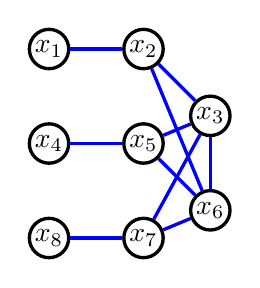
\begin{tikzpicture}[>=stealth, node distance=1.2cm]
    \tikzstyle{format} = [draw, very thick, circle, minimum size=5.0mm,
	inner sep=0pt]

	\begin{scope}
		\path[-, very thick]
			node[format] (x_1) {$x_1$}
			node[format, right of=x_1] (x_2) {$x_2$}
			node[format, below of=x_2] (x_5) {$x_5$}
			node[format, left of=x_5] (x_4) {$x_4$}
			node[format, below right of=x_2] (x_3) {$x_3$}
			node[format, below right of=x_5] (x_6) {$x_6$}
			node[format, below of=x_5] (x_7) {$x_7$}
			node[format, left of=x_7] (x_8) {$x_8$}


			(x_1) edge[blue] (x_2)
			
			(x_4) edge[blue] (x_5)
			
			(x_7) edge[blue] (x_8)
			
			(x_2) edge[blue] (x_3)
			(x_2) edge[blue] (x_6)
            (x_3) edge[blue] (x_6)

			(x_3) edge[blue] (x_5)
			(x_6) edge[blue] (x_5)
            
			(x_3) edge[blue] (x_7)
			(x_6) edge[blue] (x_7)

		;
	\end{scope}
\end{tikzpicture}
\end{center} % input answers in separate tex doc
  
\end{answertext} 

\item Which loss is easier to minimize?  Which loss is more robust to outliers?  Explain in detail.\\
\begin{answertext}{9cm}{}

The main difference between $\log p(\vec{y}, \vec{x})$ and $\log p(\vec{y} \given \vec{x})$ is the $Z$ term. Here, we have that $k'$ is very large, so computing $Z$ for $\log p(\vec{y},\vec{x})$ would perform an operation proportional to an exponential of $k'$.
% \emph{could actually determine how many parameters here if it feels like it would help}.
However, in considering $Z(\vec{x})$ in $\log p(\vec{y} \given \vec{x})$, $Z$ is parameterized by $\vec{x}$, and we only have to sum the cliques over $\vec{y}$, therefore we never have to perform any computations over the very large number of parameters $k'$, which is much more favorable. % input answers in separate tex doc
  
\end{answertext} 

\end{enumerate}

% -----------------------------------------------------------
\pagebreak
\section{Conditional Independence}
A large group of people were surveyed on their recent health. Of these, 0.20 had a fever and 0.05 had pneumonia. Among the people who had pneumonia, 0.70 had cough as a symptom and 0.50 had fever as a symptom. Among the people who had a fever, 0.40 had cough as a symptom.

Let us create a probabilistic model where the presence/absence of each of these two symptoms, cough and fever, are conditionally independent given the presence/absence of pneumonia. Using this data for the empirical probabilities of our model, answer the following questions.
\begin{enumerate}
\item Find the probability that someone has both a cough and a fever. \\
\begin{answertext}{6cm}{}

\tffalse 
% \emph{- I think, need to find a counter-example. Maybe more fundamental than that.}

Consider $A \rightarrow B \rightarrow C$. If we were to treat the model as an MRF, we would get that $A \indep C$, however, this does not hold for the DAG model, therefore, the marginal would not be the same since the distributions are different. % input answers in separate tex doc
  
\end{answertext} 
\item Find the probability that someone has pneumonia given that they have a fever but no cough. \\
\begin{answertext}{6cm}{}

\newcommand{\CI}{\mathrel{\perp\mkern-10mu\perp}}
\newcommand{\given}{~\vert~}
\newcommand{\CondInd}[3]{(#1 \CI #2 \given #3)}
% \emph{Assigned: Dimitri}
We have the following $\forall i \in [2, k-1]$ from the assumptions:
\begin{align*}
    p(x_1 \given x_2, \dots, x_k) &= p(x_1 \given x_2)\\\
    p(x_k \given x_1, \dots, x_{k-1}) &= p(x_k \given x_{k-1}) \\
    p(x_i \given \vec{x}\backslash\{x_i\}) &= p(x_i \given x_{i-1}, x_{i+1})
\end{align*}
Using Problem 5.3, we have $p(x_1, \dots, x_k) = p(x_1) \displaystyle\prod_{i=2}^n p(x_i | x_{i-1})$. There is 1 parameter for $p(x_1)$ and 2 parameters per $i$ for $p(x_i | x_{i-1})$. Therefore the number of parameters is $1 + 2(k-1) = \mathbf{2k+1}$
% Characterizing all of the conditional probabilities, we see that for $x_i$, we have 2 binary options for $i = 1, k$ and 4 binary options for $i \in [2, k-1]$. So we have that the smallest number of parameters to characterize the Gibbs sampler $p(x_1, \dots, x_k)$ is $2(2) + 4(k-2) = \mathbf{4(k-1)}$.

 % input answers in separate tex doc

\end{answertext} 

\newpage

\item Given assumptions described above, how many parameters do we need to specify the joint distribution $p(fever, cough, pneumonia)$?  \\
\begin{answertext}{6cm}{}

\tftrue

The decision boundary of a Naive Bayes classifier between two classes $Y_i$ and $Y_m$ is given by (using independence properties of Naive Bayes)
\begin{equation*}
    \log \frac{p(Y_i \given X)}{p(Y_m \given X)} = \log \frac{p(Y_i)}{p(Y_m)} + \sum_j \log \frac{p(X_j \given Y_i)}{p(X_j \given Y_m)} = constant + \sum_j g_j(X_j)
\end{equation*}
therefore, yields a linear decision boundary (in $g_j$), so Naive Bayes is a linear classifier. % input answers in separate tex doc

\end{answertext} 
\end{enumerate}


% -----------------------------------------------------------
\pagebreak
\section{Conjugate Priors}
% https://www.cs.cmu.edu/~bapoczos/Classes/ML10715_2015Fall/assignments/hw1_sol.pdf
\begin{enumerate}
\item Define what a conjugate prior is.\\
\begin{answertext}{3cm}{}  

\tffalse 
% \emph{- I think, need to find a counter-example. Maybe more fundamental than that.}

Consider $A \rightarrow B \rightarrow C$. If we were to treat the model as an MRF, we would get that $A \indep C$, however, this does not hold for the DAG model, therefore, the marginal would not be the same since the distributions are different. % input answers in separate tex doc

\end{answertext} 

\item Why are conjugate priors useful? \\
\begin{answertext}{3cm}{}

\newcommand{\CI}{\mathrel{\perp\mkern-10mu\perp}}
\newcommand{\given}{~\vert~}
\newcommand{\CondInd}[3]{(#1 \CI #2 \given #3)}
% \emph{Assigned: Dimitri}
We have the following $\forall i \in [2, k-1]$ from the assumptions:
\begin{align*}
    p(x_1 \given x_2, \dots, x_k) &= p(x_1 \given x_2)\\\
    p(x_k \given x_1, \dots, x_{k-1}) &= p(x_k \given x_{k-1}) \\
    p(x_i \given \vec{x}\backslash\{x_i\}) &= p(x_i \given x_{i-1}, x_{i+1})
\end{align*}
Using Problem 5.3, we have $p(x_1, \dots, x_k) = p(x_1) \displaystyle\prod_{i=2}^n p(x_i | x_{i-1})$. There is 1 parameter for $p(x_1)$ and 2 parameters per $i$ for $p(x_i | x_{i-1})$. Therefore the number of parameters is $1 + 2(k-1) = \mathbf{2k+1}$
% Characterizing all of the conditional probabilities, we see that for $x_i$, we have 2 binary options for $i = 1, k$ and 4 binary options for $i \in [2, k-1]$. So we have that the smallest number of parameters to characterize the Gibbs sampler $p(x_1, \dots, x_k)$ is $2(2) + 4(k-2) = \mathbf{4(k-1)}$.

 % input answers in separate tex doc

\end{answertext} 

\item Show that the Gamma distribution is a conjugate prior of the exponential distribution. That is, show that if $x \sim \text{Exp}(\lambda)$ and $\lambda \sim \text{Gamma}(\alpha, \beta)$, then $p(\lambda | x) \sim \text{Gamma}(\alpha^*, \beta^*)$ for some $\alpha^*$, $\beta^*$. \\
\begin{answertext}{6cm}{}

\tftrue

The decision boundary of a Naive Bayes classifier between two classes $Y_i$ and $Y_m$ is given by (using independence properties of Naive Bayes)
\begin{equation*}
    \log \frac{p(Y_i \given X)}{p(Y_m \given X)} = \log \frac{p(Y_i)}{p(Y_m)} + \sum_j \log \frac{p(X_j \given Y_i)}{p(X_j \given Y_m)} = constant + \sum_j g_j(X_j)
\end{equation*}
therefore, yields a linear decision boundary (in $g_j$), so Naive Bayes is a linear classifier. % input answers in separate tex doc

\end{answertext} 
\end{enumerate}

\pagebreak
\section{Gibbs Sampling and the Semi-Graphoid Axioms}

\begin{enumerate}
\item Assume a joint distribution $p(x_1, \ldots, x_k)$ over binary random variables $X_1, \ldots, X_k$.
What's the size of the joint probability table?\\
\begin{answertext}{3cm}{}

\tffalse 
% \emph{- I think, need to find a counter-example. Maybe more fundamental than that.}

Consider $A \rightarrow B \rightarrow C$. If we were to treat the model as an MRF, we would get that $A \indep C$, however, this does not hold for the DAG model, therefore, the marginal would not be the same since the distributions are different. % input answers in separate tex doc

\end{answertext}

\item Assume $(X_1 {\perp\!\!\!\perp} X_3, \ldots, X_k \mid X_2)$, $(X_k {\perp\!\!\!\perp} X_1, \ldots, X_{k-2} \mid X_{k-1})$, and $(X_i {\perp\!\!\!\perp} X_1, \ldots, X_{i-2}, X_{i+2}, \ldots, X_k \mid X_{i-1}, X_{i+1})$ for each $i = 2, \ldots, k-1$.  What's the smallest number of parameters we would need to specify to create a Gibbs sampler for $p(x_1, \ldots, x_k)$?\\
\begin{answertext}{6cm}{}

\newcommand{\CI}{\mathrel{\perp\mkern-10mu\perp}}
\newcommand{\given}{~\vert~}
\newcommand{\CondInd}[3]{(#1 \CI #2 \given #3)}
% \emph{Assigned: Dimitri}
We have the following $\forall i \in [2, k-1]$ from the assumptions:
\begin{align*}
    p(x_1 \given x_2, \dots, x_k) &= p(x_1 \given x_2)\\\
    p(x_k \given x_1, \dots, x_{k-1}) &= p(x_k \given x_{k-1}) \\
    p(x_i \given \vec{x}\backslash\{x_i\}) &= p(x_i \given x_{i-1}, x_{i+1})
\end{align*}
Using Problem 5.3, we have $p(x_1, \dots, x_k) = p(x_1) \displaystyle\prod_{i=2}^n p(x_i | x_{i-1})$. There is 1 parameter for $p(x_1)$ and 2 parameters per $i$ for $p(x_i | x_{i-1})$. Therefore the number of parameters is $1 + 2(k-1) = \mathbf{2k+1}$
% Characterizing all of the conditional probabilities, we see that for $x_i$, we have 2 binary options for $i = 1, k$ and 4 binary options for $i \in [2, k-1]$. So we have that the smallest number of parameters to characterize the Gibbs sampler $p(x_1, \dots, x_k)$ is $2(2) + 4(k-2) = \mathbf{4(k-1)}$.

 % input answers in separate tex doc

\end{answertext}

\item Assume conditional independences as in the previous question.  Use the chain rule of probability and the graphoid axioms to write down the likelihood for the model such that only a polynomial number of parameters (in $k$) are used.\\
\begin{answertext}{6cm}{}

\tftrue

The decision boundary of a Naive Bayes classifier between two classes $Y_i$ and $Y_m$ is given by (using independence properties of Naive Bayes)
\begin{equation*}
    \log \frac{p(Y_i \given X)}{p(Y_m \given X)} = \log \frac{p(Y_i)}{p(Y_m)} + \sum_j \log \frac{p(X_j \given Y_i)}{p(X_j \given Y_m)} = constant + \sum_j g_j(X_j)
\end{equation*}
therefore, yields a linear decision boundary (in $g_j$), so Naive Bayes is a linear classifier. % input answers in separate tex doc

\end{answertext} 
\end{enumerate}

\end{document}
